\chapter{范畴论基础}
\section{范畴与态射}
概括地说,范畴是由对象及其间的态射组成的数学结构,从对象$X$到对象$Y$的态射$f$习惯以箭头来描述
\[
    X \xrightarrow{f} Y
\]
函子视作范畴间保持箭头结构的某种“映射”,函子之间的关系由自然变换描述。

数学中考虑的范畴经常以一类特定的结构为对象,例如群,环,向量空间,偏序集,拓扑空间等,范畴中的态射经常是保结构的映射,如群同态,连续映射等。函子与自然变换在这种种结构之间搭起桥梁。范畴论的本意不止于研究它们各自的性质。

    范畴视角的特色正在于重视关联甚于数学对象本身,并以同构代替严格等式。

    实际上,范畴里的对象未必是建立在集合上的结构,而态射也未必是映射。

    \begin{center}
        \begin{tabular}{|c|c|c|c|c|}\hline
                & 拓扑学 & 量子物理 & 数理逻辑 & 计算机科学   \\
                & (配边理论) & & (形式演绎系统) & (带类型的$\lambda$演算)  \\ \hline
            对象 & 流形 & 物理系统 & 命题 & 资料形态 \\ \hline
            态射 & 配边关系 & 过程 & 证明 & 程序 \\  \hline
        \end{tabular}
    \end{center}
    自然学科终归需要实践来检验。

    实用中往往会考虑带有特殊结构的范畴。幺半范畴是最常见的结构之一,其中具有类似于乘法的操作。

    集合的大小对范畴的性质有实在的影响。

\begin{Def}[范畴$\mathcal{C}$]指:

    \begin{enumerate}
        \item 集合$\Obj(\mathcal{C})$,其元素称作$\mathcal{C}$的 \emph{对象}
        \item 集合$\Mor({\mathcal{C}})$,其元素称作$\mathcal{C}$的 \emph{态射},配上一对映射
        \begin{center}
            $\begin{tikzcd} \Mor(\mathcal{C}) \arrow[yshift=-0.5ex, r, "t"'] \arrow[yshift=0.5ex, r, "s"] & \Obj(\mathcal{C}) \end{tikzcd}$
        \end{center}
        其中$s,t$分别给出态射的\emph{来源}和\emph{目标}。对于$X,Y\in \Obj(\mathcal{C})$,习惯记 $\Hom_{\mathcal{C}}(X,Y):=s^{-1}(X)\cap t^{-1}(Y)$或简记为$\Hom(X,Y)$,称为$\Hom$-集,其元素称为从$X$到$Y$上的态射。
        
        (从$X$出发的态射和到达$Y$的态射的交集)

        \item 任意对象$X$给定元素$\identity_X\in \Hom_{\mathcal{C}}(X,X)$,称为$X$到自身的\emph{恒等态射}。
        \item $\forall X,Y,Z \in \Obj(\mathcal{C})$,给定态射间的 \emph{合成映射}
        \begin{align*}
            \circ: \Hom_{\mathcal{C}}(Y,Z)\times \Hom_{\mathcal{C}}(X,Y) &\longrightarrow \Hom_{\mathcal{C}}(X,Z) \\
            (f,g) & \longmapsto f\circ g  \\
        \end{align*}
        不致混淆时常将 $f \circ g$简记为$fg$,它满足
        \begin{enumerate}
            \item 结合律: $\forall $态射$h,g,f\in \Mor(\mathcal{C})$,若合成$f(gh)$和$(fg)h$都有定义,则
            \[f(gh)=(fg)h\]
            \item $\forall $态射$f\in \Hom_{\mathcal{C}}(X,Y)$有
            \[
                f\circ \identity_X=f=\identity_Y \circ f
            \]
        \end{enumerate}
    \end{enumerate}
\end{Def}
\begin{Rmk}.
    \begin{itemize}
        \item 注意到$\identity_X$被其性质唯一确定。对象与态射集皆空的范畴称为\emph{空范畴},记为$\mathbf{0}$.
        \item 一般也将 $f \in \Hom_{\mathcal{C}}(X,Y)$写作$f:X\rightarrow Y$或$X\xrightarrow{f}Y$,故态射有时又叫作箭头。态射的合成对应于箭头的头尾衔接。图表加箭头是讨论范畴的方便语言。其中最常用的是\emph{交换图表}的概念,“交换”意指箭头的合成殊途同归,例如:
        \[\begin{tikzcd}
            X \arrow[rr, "f"] \arrow[rd, "h"'] & & Y \arrow[ld, "g"] \\
            & Z &
        \end{tikzcd}
        \qquad
        \begin{tikzcd}
            A \arrow[r, "u"] \arrow[d,"x"] & B \arrow[d,"v"] \\
            C \arrow[r,"y"]  & D    \\
        \end{tikzcd}
        \]
        的交换性分别等价于$gf=h$和$vu=yx$。态射的名称$f,g$等自明或者不重要,则常可以从图表中省略。
        \item 对于态射$f:X\rightarrow Y,\exists g:Y\rightarrow X\Rightarrow fg=\identity_Y \wedge gf= \identity_X$,则称$f$是同构(或称可逆,写作$f:X\xrightarrow{\sim}Y$),$g$称为$f$的\emph{逆},从恒等态射的性质易见逆若存在则唯一。从$X$到$Y$的同构集记为$\Isom_{\mathcal{C}}(X,Y)$.
        \item 记$\End_{\mathcal{C}}:=\Hom_{\mathcal{C}}(X,X), \Aut_{\mathcal{C}}(X):=\Isom_{\mathcal{C}}(X,X)$,分别称作$X$的自同态集和自同构集。这些集合在二元运算$\circ$下封闭:用代数的语言来说,$\End(X)$是幺半群,$\Aut(X)$是群。
    \end{itemize}
\end{Rmk}

\begin{Def}[子范畴] 称$\mathcal{C}'$是$\mathcal{C}$的\emph{子范畴},如果满足四条件:
    \begin{enumerate}
        \item $\Obj(\mathcal{C}') \subset \Obj(\mathcal{C})$
        \item $\Mor(\mathcal{C}') \subset \Mor(\mathcal{C})$,并保持恒等态射
        \item 来源/目标映射 
        $\begin{tikzcd}
            \Mor(\mathcal{C}')
                \arrow[yshift=-0.5ex,r,"t"']
                \arrow[yshift= 0.5ex,r,"s" ] &
            \Obj(\mathcal{C}')
        \end{tikzcd}$
        是由$\mathcal{C}$限制而来的
        \item $\mathcal{C}'$中态射的合成也是由$\mathcal{C}$限制而来的
    \end{enumerate}
    简而言之,任意$\mathcal{C}$中的对象$X,Y$,有包含关系$\Hom_{\mathcal{C}'}(X,Y)\subset \Hom_{\mathcal{C}}(X,Y)$,它与态射的合成兼容。如果$Hom_{\mathcal{C}'}(X,Y)=\Hom_{\mathcal{C}}(X,Y)$则称$\mathcal{C}'$是全子范畴。
    
\end{Def}

\begin{Def}[$\mathcal{U}$-范畴,$\mathcal{U}$-小范畴].

    范畴$\mathcal{C}$对于$\forall X,Y\in \Obj(\mathcal{C})$,集合$\Hom_{\mathcal{C}}(X,Y)$都是$\mathcal{U}$-小集(局部$\mathcal{U}$-小范畴)。

    如果态射集$\Mor(\mathcal{C})$也是$\mathcal{U}$-小集,则称为$\mathcal{U}$-小范畴
\end{Def}

\begin{Rmk}.

    范畴$\mathcal{C}$是$\mathcal{U}$-小范畴当且仅当它是 $\mathcal{U}$-范畴且$\Obj(\mathcal{C})$是$\mathcal{U}$-小集。因为$X\mapsto id_X$将$\Obj(\mathcal{C})$嵌入$\Mor(\mathcal{C})$.

    将群、环、空间等其它结构称为$\mathcal{U}$-群(环、空间),如果它们作为集合是一个$\mathcal{U}$-集合。不致混淆时,也简称作小集,小群等等。
\end{Rmk}

\begin{Cvs}[\label{con:U-small}]
    选定宇宙后,若不另外说明,将略去符号$\mathcal{U}$将集合、群等理解为$\mathcal{U}$-集(群)等。所论的范畴如不另外说明都是$\mathcal{U}$-范畴。
\end{Cvs}

\begin{Exap}[几个基本的范畴的例子].
    \begin{enumerate}
        \item 预序集等同于任意两个对象之间至多有一个态射的范畴:对于预序集$(P,\leq )$,定义范畴使得其对象集为$P$,而存在态射$p\rightarrow p' \Leftrightarrow p\leq p'$,此时这样的态射唯一。特别地,根据对有限序数的递归定义,任意$n\in \mathbb{Z}_{\geq 0}$视为序数等同于全序集$\{0,...,n-1\}$,而$0=\emptyset $。相应的范畴记为$\mathbf{n}$,其结构可以形象地表为
        \[
            0\rightarrow 1\rightarrow ... \rightarrow (n-1) \text{(略去恒等态射)}
        \]
        特别地,$0$给出空范畴$\mathbf{0}$,$1$给出恰有一个对象和一个态射的范畴$\mathbf{1}$.
        \item 令$\cate{Set}$为所有集合构成的范畴,对象$X,Y$之前的态射定义为映射$X\rightarrow Y$。态射的合成就是映射的合成,恒等态射就是映射的合成,恒等态射就是恒等映射。这是$\mathcal{U}$-范畴。
        \item 带基点的集合范畴$\cate{Set}_\bullet$。对象是所有$(X, x)$,其中$X$是集合$x\in X$(基点),从$(X,x)\rightarrow (Y,y)$的态射是满足$f(x)=y$的映射$f:X\rightarrow Y$
        \item 令$\cate{Grp}$是所有群构成的范畴,对象之间的态射定义为群同态,态射的合成与恒等态射定义与$\cate{Set}$相同。
        \[
            f(xy)=f(x)f(y)
        \]
        \item 令$\cate{Ab}$为所有交换群(Abel群,二元运算用加法$+$)构成的范畴,态射与$\cate{Grp}$的情形相同。它是$\cate{Grp}$的全子范畴。注意到交换群的同态可以相加(复合),因此对于任意两个交换群$X,Y$,同态集$\Hom(X,Y)$不仅是一个集合,它还具有交换群的结构($G,+$),这使得合成映射$\Hom(Y,Z)\times \Hom(X,Y)\rightarrow \Hom(X,Z)$满足双线性:
        \[
            (f+g)h=fh+gh, \quad h(f+g)=hf+hg
        \]
        这是$\cate{Ab}$-范畴的一个特殊情形。
        \[
            (f+g)(xy)=f(g(x)g(y))=f(g(x))f(g(y))=(f+g)(x)\cdot (f+g)(y)
        \]

        \item 令$\cate{Top}$为所有拓扑空间构成的范畴,空间皆假定为 Hausdorff 的,态射定义为连续映射,合成与恒等态射的定义同上;类似的定义带基点的拓扑空间$\cate{Top}_\bullet$。我们也希望赋予同态集$\Hom(X,Y)$额外的结构,例如紧开拓扑,使得$\Hom(Y,Z)\times \Hom(X,Y)\rightarrow \Hom(X,Z)$成为连续映射;更希望能有自然的同构
        \[
            \Hom(X\times Y, Z) \xrightarrow{\sim}\Hom(X,\Hom(Y,Z))
        \]
        相关的点集拓扑问题颇为棘手,为了在确保良好的范畴性质的同时容许充分广的拓扑空间,在同伦论里一般选用$\cate{Top}$的一个子范畴$\cate{CGHaus}$,称为紧生成 Hausdorff 空间范畴
        \item 选定一个域$\Bbbk$,令$\cate{Vect(\Bbbk)}$为$\Bbbk$上的所有向量空间构成的范畴,态射为线性映射。类此定义有限维向量空间范畴$\cate{Vect}_{f}(\Bbbk)$,它是$\cate{Vect}(\Bbbk)$的全子范畴
        \item 给定集合$S$,定义相应的离散范畴$\cate{Disc}(S)$:其对象集为$S$而态射仅有恒等态射$\{\identity_x:x\in S\}$
    \end{enumerate}
\end{Exap}
\begin{Rmk}如果不用约定 \ref{con:U-small} 而直接考虑所有集合,所有群等等构成的范畴,则会面临悖论,因为所有集合的全体并不构成集合。常见的一种做法是区分类和集,并要求对象全体成一个类$\Obj({\mathcal{C}})$,而任一个态射集$\Hom_{\mathcal{C}}(X,Y)$是集合。用ZFC来考虑较为迂回,而NBG集合论则特别适应与这个编发。将真类引入范畴论公理会造成不少麻烦,之后要讨论的函子范畴是一个例子。因此我们宁可引入宇宙的概念,并假设所考察的数学对象都是$\mathcal{U}$-小的。
\end{Rmk}

    单射和满射的概念有自然的范畴论推广

\begin{Def}[单态射,满态射]$X,Y$为范畴$\mathcal{C}$中的对象,$f\in \Hom_{\mathcal{C}}(X,Y)$
    \begin{enumerate}
        \item 单态射 任何对象$Z$和任一对态射$g,h:Z\rightarrow X$有$fg=fh\Leftrightarrow g=h$ 左消去律;
        \item 满态射 任何对象$Z$和任一对态射$g,h:Y\rightarrow Z$有$gf=hf\Leftrightarrow g=h$ 右消去律;
    \end{enumerate}
    如存在$g$使得$gf=id_X$,则称$f$左可逆而$g$是它的一个左逆;类似的可以定义右逆。左可逆蕴含单,右可逆蕴含满。态射可逆当且仅当它左右皆可逆。
\end{Def}

\begin{Exap}[常用范畴中的单性与满性].

    在范畴$\cate{Set}, \cate{Grp}, \cate{Vect}(\Bbbk)$中,态射的单性与满性分别等价于集合论意义下的单射和满射,而且既单又满的态射恰好是同构。对其它范畴则略有区别。在$\cate{Top}$中,态射$f:X\rightarrow Y$有稠密的像便是满态射。而在复拓扑向量空间范畴$\cate{TopVect}(\mathbb{C})$中,存在许多连续线性映射$f:V\rightarrow W$,使得$f$是双射而非开映射,这样的态射既单且满,却不是同构。
\end{Exap}

\begin{Def}[广群]
    若一个范畴 $\mathcal{C}$中的所有态射都可逆,则称之为\emph{广群}。
\end{Def}

    只有一个对象的范畴与幺半群一一对应:相应的幺半群是$\End(X),x$是唯一对象。群无非是只有一个对象的广群。由于广群里的箭头都是同构,它适合用来表述数学对象的分类问题。???

\begin{Exap}[基本广群]
    设$X$是拓扑空间,两点$x,y$之间的道路意指连续映射$f:[0,1]\rightarrow X,f(0)=x,f(1)=y$.道路的合成无非是头尾相接:对于$x,y,z\in X$和道路$f(x\rightarrow y),f'(y\rightarrow z)$,定义$x\rightarrow z$的道路$f''$为:
    \[
        f''(t)=
        \begin{cases}
            f(2t),      & 0\leq t\leq \frac{1}{2}   \\
            f'(2t-1),   & \frac{1}{2} < t \leq 1    \\
        \end{cases}
    \]

    两条$x,y$之间的道路$f,f'$称为(定端)同伦的,如果存在连续映射$F:[0,1]^2\rightarrow X$使得对每个$t\in [0,1], F(\cdot,t)$都是$x,y$之间的道路,而且$F(\cdot,0)=f, F(\cdot, 1)=f'$。同伦构成一个等价关系。易见道路的合成可以在同伦类的层次定义。
    \begin{center}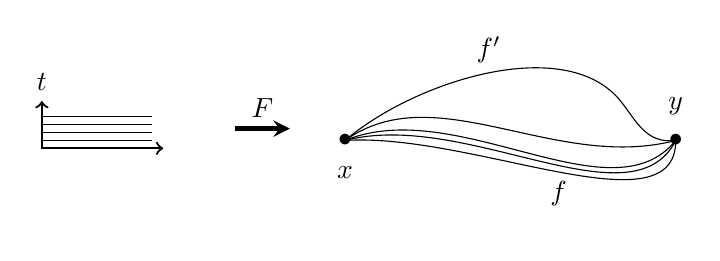
\begin{tikzpicture}[xscale=0.7, yscale=0.5]
        \draw [thick, <->] (1.5,6.2) node [above] {$t$} -- (1.5,5) -- (3.7,5);
        \draw (1.5,5.2) -- (3.5,5.2);
        \draw (1.5,5.4) -- (3.5,5.4);
        \draw (1.5,5.6) -- (3.5,5.6);
        \draw (1.5,5.8) -- (3.5,5.8);

        \draw [-stealth, ultra thick] (5, 5.5) -- (6,5.5) node[midway, above] {$F$};
        
        \coordinate (x) at (7, 5.2);
        \coordinate (y) at (13, 5.2);
        \node[label=below:$x$] (x) at (7, 5.2){$\bullet$};
        \node[label=above:$y$] (y) at (13, 5.2){$\bullet$};
        \draw (x.center) to [out=5, in=-90, edge node={node[below] {$f$}}] (y.center);
        \draw (x.center) to [out=20, in=-110] (y.center);
        \draw (x.center) to [out=30, in=-120] (y.center);
        \draw (x.center) to [out=45, in=-160] (y.center);
        \draw (x.center) to [out=50, in=-240, edge node={node[above] {$f'$}}] ++(5, 1) to [out=-60, in=-170] (y.center); 
    \end{tikzpicture}\end{center}
    空间$X$的基本广群$\Pi_1(X)$定义为如下范畴,其对象是$X$中的点,对任意$x,y \in X$,态射集$\Hom(x,y)$定义为所有从$x$到$y$的道路类;态射的合成定义为道路类的合成,而恒等态射$\identity_x$由静止道路$\forall t, \identity_x(t)=x$表示。对于给定的态射$f:x\rightarrow y$(同伦类中的某个代表元),其逆可以取为反向道路$f^{-1}:=f(1-t),t\in[0,1]$。

    可以验证这些操作都是良定的,并使得$\Pi_1(X)$成为广群。注意到$\Aut(X)=\Hom(x,x)$正好是以$x$为基点的\emph{基本群}$\pi_1(X,x)$.
\end{Exap}
    基本群是拓扑学中重要的不变量,它为每个空间$X$指定一个相应的代数结构(群)。 基本广群可以视为再高一阶的不变量:它为$X$指定一个范畴。但是应当注意还有大量拓扑信息被$\Pi_1(X)$的范畴结构遗漏了:除了道路的同伦类,还应该计入道路间的同伦等价,还可以设想同伦之间更有同伦,直至无穷。凡此种种都必须以更高阶的范畴语言反映。???

\begin{Def}[反范畴]任意范畴$\mathcal{C}$,其反范畴$\mathcal{C}^{\text{op}}$定义为:
    \begin{itemize}
        \item $\Obj(\mathcal{C}^{\text{op}})=\Obj(\mathcal{C})$
        \item $\forall X,Y \in \Obj(\mathcal{C}), \Hom_{\mathcal{C}^{\text{op}}}(X,Y):=\Hom_{\mathcal{C}}(Y,X)$
        \item $f \in \Hom_{\mathcal{C}^{\text{op}}}(Y,Z), g\in \Hom_{\mathcal{C}^{\text{op}}}(X,Y)$在$\mathcal{C}^{\text{op}}$中的合成$f \circ^{\text{op}}g$定义为$\mathcal{C}$中的反向合成$g\circ f$
        \item 恒等态射定义等同$\mathcal{C}$
    \end{itemize}
    容易验证$\mathcal{C}^{\text{op}}$满足范畴定义,且$(\mathcal{C}^{\text{op}})^{\text{op}}=\mathcal{C}$。
\end{Def}
    简而言之,$\mathcal{C}^{\text{op}}$的构造就是反转箭头,反转之后的范畴论公理依然成立,范畴论中的这种对称性也称作对偶原理。例如:$\mathcal{C}^{\text{op}}$中的单态射无非是$\mathcal{C}$中的满态射。

\section{函子与自然变换}

\begin{Def}[函子]设$\mathcal{C}',\mathcal{C}$为范畴。一个函子$F:\mathcal{C}'\rightarrow C$指:
    \begin{enumerate}
        \item 对象间的映射 $F:\Obj(\mathcal{C}')\rightarrow \Obj(\mathcal{C})$
        \item 态射间的映射 $F:\Mor(\mathcal{C}')\rightarrow \Mor(\mathcal{C})$ 使得
        \begin{itemize}
            \item $F$的来源和目标映射可交换$sF=Fs, tF=Ft$,等价的说法是$\forall X,Y\in \Obj(\mathcal{C}')$都有映射$F:\Hom_{\mathcal{C}'}(X,Y)\rightarrow \Hom_{\mathcal{C}}(FX,FY)$
            \item $F(g\circ f)=F(g)\circ F(f); F(\identity_X)=\identity_{FX}$
        \end{itemize}
    \end{enumerate}
    对于$F:\mathcal{C}_1\rightarrow \mathcal{C}_2, G:\mathcal{C}_2\rightarrow \mathcal{C}_3$,合成函子$G\circ F:\mathcal{C}_1\rightarrow \mathcal{C}_3$的定义是显然的:取合成映射
    \begin{gather*}
        \Obj(\mathcal{C}_1)\xrightarrow{F} \Obj(\mathcal{C}_2)\xrightarrow{G} \Obj(\mathcal{C}_3)       \\
        \Mor(\mathcal{C}_1)\xrightarrow{F} \Mor(\mathcal{C}_2)\xrightarrow{G}\Mor(\mathcal{C}_3)    \\
    \end{gather*}
\end{Def}
旧文献常将上述函子称为$\mathcal{C}'$到$\mathcal{C}$的共变函子,形如$F:(\mathcal{C}')^{\text{op}}\rightarrow \mathcal{C}$的函子为反变函子。

\begin{Rmk}
    从$\mathcal{C'}$到$\mathcal{C}$和从$(\mathcal{C}')^{\text{op}}$到$\mathcal{C}^{\text{op}}$的函子是一回事。为区分,对于函子$F:\mathcal{C}'\rightarrow \mathcal{C}$,反范畴间的相应函子记为$F^{\text{op}}:(\mathcal{C}')^{\text{op}}\rightarrow \mathcal{C}^{\text{op}}$
\end{Rmk}

\begin{Def}[函子的满性,忠实性,全性]
    对于函子$F:\mathcal{C}'\rightarrow \mathcal{C}$
    \begin{enumerate}
        \item 本质满的:若$\mathcal{C}$中任一对象都同构于某个$FX$
        \item 忠实的: 若$\forall X,Y\in \Obj(\mathcal{C}')$,映射$\Hom_{\mathcal{C}'}(X,Y)\rightarrow \Hom_{\mathcal{C}}(FX,FY)$都是单射
        \item 全的:上述映射对$\forall X,Y\in \Obj(\mathcal{C}')$都是满射
    \end{enumerate}
\end{Def}

\begin{Exap}[函子].
    \begin{enumerate}
        \item 子范畴$\mathcal{C}'\subset \mathcal{C}$给出一个包含函子$\iota:\mathcal{C}' \hookrightarrow \mathcal{C}$;包含函子总是忠实的,它是全函子当且仅当$\mathcal{C}'$是全子范畴。取$\mathcal{C}'=\mathcal{C}$就得到恒等函子$\identity_{\mathcal{C}}:\mathcal{C}\rightarrow \mathcal{C}$
        \item 考虑群范畴$\cate{Grp}$.$\forall$群$G$,总是可以忘掉$G$的群结构而视之为集合,群同态当然也可以视为集合间的映射,此程序给出\emph{忘却函子}$\cate{Grp}\rightarrow \cate{Set}$。类似地给出忘却其它结构的忘却函子
        $\cate{Top}\rightarrow \cate{Set}$(忘却空间的拓扑结构),$\cate{Vect}(\Bbbk)\rightarrow \cate{Ab}$(忘掉$\Bbbk$-向量空间$V$的纯量乘法,只看它的加法群$(V,+)$)等等。这类函子显然忠实而非全。
        \item 考虑域$\Bbbk$上的向量空间范畴$\cate{Vect}(\Bbbk)$。对于任意$\Bbbk$-向量空间$V$,定义其对偶空间
        \[
            V^{\vee}:=\Hom_{\Bbbk}(V,\Bbbk)=\{\Bbbk \text{-线性映射}V\rightarrow \Bbbk\}
        \]
        任一线性映射$f:V_1\rightarrow V_2$诱导对偶空间的反向映射
        \begin{gather*}
            f^{\vee}:V_{2}^{\vee}\rightarrow V_1^{\vee} \\
            [\lambda:V_2 \rightarrow \Bbbk] \mapsto \lambda \circ f
        \end{gather*}
        易见$D:V\mapsto V^{\vee}, f\mapsto f^{\vee}$定义了函子$D:\cate{Vect}(\Bbbk)^{\text{op}}\rightarrow \cate{Vect}(\Bbbk)$,可以验证$D$是忠实的。根据反函子的定义合成函子$DD^{\text{op}}: \cate{Vect}(\Bbbk)\rightarrow \cate{Vect}(\Bbbk)$

        将$D$限制于有限维向量空间,得到函子$D:\cate{Vect}_f(\Bbbk)^{\text{op}}\rightarrow \cate{Vect}_f(\Bbbk)$和$DD^{\text{op}}:\cate{Vect}_{f}(\Bbbk)\rightarrow \cate(Vect)_{f}(\Bbbk)$,分别称为对偶和双对偶函子。
        
        \item 对于任意群$G$,定义导出子群$G_{\text{der}}$为子集$\{xyx^{-1}:x,y\in G\}$生成的正规子群。商群$G/G_{\text{der}}$是交换群,称作$G$的Abel化。对于任意群同态$\varphi:G\rightarrow H$,从定义可以看出$\varphi(G_{\text{der}})\subset H_{\text{der}}$,因此$\varphi$诱导出交换群的同态$\bar{\varphi}:G/G_{\text{der}}\rightarrow H/H_{\text{der}}$。容易验证$G\mapsto G/G_{\text{der}}, \varphi \mapsto \bar{\varphi}$定义了Abel化函子$\cate{Grp}\rightarrow \cate{Ab}$。Abel化函子不是忠实函子。
        \item 对任意带点拓扑空间$(X,x)$指定基本群$\pi_1(X,x)$,给出了函子$\cate{Top}_{\bullet}\rightarrow \cate{Grp}$。代数拓扑学中还有许多例子,例如空间的同调群$X\mapsto H_n(X;Z)$给出了一族函子$H_n:\cate{Top}\rightarrow \cate{Ab}$,其中$n\in \mathbb{Z}_{\geq 0}$,上同调群给出函子$H^n:\cate{Top}^{\text{op}}\rightarrow \cate{Ab}$。
    \end{enumerate}
\end{Exap}

\begin{Def}[自然变换,或函子间的态射] 函子$F,G:\mathcal{C}'\rightarrow \mathcal{C}$之间的自然变换$\theta$是一族态射
    \[
        \theta_X \in \Hom_{\mathcal{C}}(FX,GX), X\in \Obj(\mathcal{C}')
    \]
    使得下图所有$\mathcal{C}'$中的态射交换
    \begin{center}\begin{tikzcd}
        FX \arrow[r, "\theta_X"] \ar[d, "Ff"'] & GX \arrow[d, "Gf"] \\
        FY \arrow[r, "\theta_Y"'] & GY .
    \end{tikzcd}\end{center}
    上述自然变换写作$\theta:F \to G$,或图解为
    \[\begin{tikzcd}
            \mathcal{C}' \arrow[bend left=50, r, "F", ""' name=U] \arrow[bend right=50, r, "G"', "" name=D] & \arrow[Rightarrow, to path=(U)--(D) \tikztonodes, "\theta"] \mathcal{C}
    \end{tikzcd}\]
    上述带有双箭头$\Rightarrow$的图表有时也被称为2-胞腔,一种兴许更有益的看法是设想$\theta $为从$F$到$G$的一个同伦。
\end{Def}
\begin{Cvs}.
    我们也将自然变换$\theta:F \to G$称为从函子$F$到$G$的态射。实用中经常会省略严格的范畴论框架,只说态射$\theta_X:FX\to GX$对于变元$X$是\emph{自然}的,\emph{典范}的,或称满足\emph{函子性}。实践中经常把自然同构直接写成等号$=$。
\end{Cvs}

    几种自然变换的操作,包括纵、横两种合成
    \begin{itemize}
        \item 纵合成: 考虑$\mathcal{C}'$到$\mathcal{C}$的三个函子间的态射$\theta:F\to G,\psi:G\to H$。纵合成$\psi \circ \theta :=\{\psi_X \circ \theta_X :X \in \Obj(\mathcal{C})\}$,图解:
        \[\begin{tikzcd}
            \mathcal{C}'
                \arrow[bend left=70, rr, "F", ""' name=U]
                \arrow[rr, "G" name=MM, ""' name = M]
                \arrow[bend right=70, rr, "" name=D, "H"'] & &
            \arrow[Rightarrow, to path=(U) -- (MM) \tikztonodes, "\theta"]
            \arrow[Rightarrow, to path=(M) -- (D) \tikztonodes, "\psi"]
            \mathcal{C}
        \end{tikzcd}
        \quad \text{合成为} \quad
        \begin{tikzcd}
            \mathcal{C}'
                \arrow[bend left = 50, rr, "F", ""' name = U]
                \arrow[bend right = 50, rr, "" name = D, "H"']  &&
            \arrow[Rightarrow, to path = (U) -- (D) \tikztonodes, "\psi \circ \theta"]
            \mathcal{C}
        \end{tikzcd}\]
        \item 横合成:考虑函子
        \begin{tikzcd}
            \mathcal{C}''
                \arrow[bend left = 30, r, "F_1"]
                \arrow[bend right = 30, r, "F_2"] &
            \mathcal{C}'
                \arrow[bend left = 30, r, "G_1"]
                \arrow[bend right = 30, r, "G_2"] &
            \mathcal{C}
        \end{tikzcd}
        及态射$\theta:F_1 \to F_2, \psi: G_1 \to G_2$。现定义横合成$\psi\circ \theta: G_1 \circ F_2 \to G_2 \circ F_2$。注意到对所有$X\in \Obj(\mathcal{C}'')$,根据$\psi$的自然性,图表
        \[\begin{tikzcd}
            G_1 F_1(X)
                \arrow[r, "{\psi_{F_1 X}}"]
                \arrow[d, "{G_1(\theta_X)}"'] &
            G_2 F_1(X)
                \arrow[d, "{G_2(\theta_X)}"]  \\
            G_1 F_2(X)
                \arrow[r, "{\psi_{F_2 X}}"'] &
            G_2 F_2(X)
        \end{tikzcd}\]
        交换。对角合成$\searrow$记作$(\psi \circ \theta)_X:G_1 F_1 (X) \to G_2 F_2 (X)$, 此即所求的横合成,我们马上会证明它的自然性。图解:
        \[\begin{tikzcd}
            \mathcal{C}''
                \arrow[bend left = 50, r, "F_1", ""' name = U1]
                \arrow[bend right = 50, r, "" name = D1,"F_2"'] &
            \mathcal{C}'
                \arrow[bend left = 50, r, "G_1", ""' name = U2]
                \arrow[bend right = 50, r, "" name = D2, "G_2"'] &
            \mathcal{C}
            \arrow[Rightarrow, to path = (U1) -- (D1) \tikztonodes, "\theta"]
            \arrow[Rightarrow, to path = (U2) -- (D2) \tikztonodes, "\psi"]
        \end{tikzcd}
        \quad \text{合成为} \quad
        \begin{tikzcd}
            \mathcal{C}''
                \arrow[bend left = 50, rr, "{G_1 F_1}", ""' name = U]
                \arrow[bend right = 50, rr, "" name = D, "{G_2 F_2}"'] & &
            \mathcal{C}
            \arrow[Rightarrow, to path = (U) -- (D) \tikztonodes, "{\psi \circ \theta}"]
        \end{tikzcd}\]
        \item 横合成的特例
        \[\begin{tikzcd}
            \mathcal{C}_1
                \arrow[r, "H"] &
            \mathcal{C}_2
                \arrow[bend left = 50, r, "F", ""' name = U]
                \arrow[bend right = 50, r, "" name = D, "G"'] &
            \mathcal{C}_3
                \arrow[r, "K"]  &
            \mathcal{C}_4
            \arrow[Rightarrow, to path = (U)--(D) \tikztonodes, "\theta"]
        \end{tikzcd}\]
        对左边三项:$\theta H:FH\to GH$简记横合成$\theta\circ\identity_{H}$;具体地说,$(\theta H)_X = \theta_{HX}:FH(X)\to GH(X)$;类似地处理右三项:$K\theta :KF\to KG$为横合成$\identity_{K}\circ \theta$,我们有$(K\theta)_X=K(\theta_X):KF(X)\to KG(X)$
    \end{itemize}

\Rmk{这里使用了同一个符号$\circ$表示纵横合成,如有混淆之虞将另作说明}

\begin{Lem}横纵合成$\{(\psi \circ \theta)_X\}_X$都是函子间的态射,而且各自满足严格结合律$(\phi \circ \psi) \circ \theta = \phi \circ (\psi \circ \theta)$。横纵合成之间满足关系:对于图表
    \[\begin{tikzcd}
        \mathcal{C}_1
            \arrow[bend left = 50, rr, ""' name = U1]
            \arrow[rr, "" name = UM1, ""' name = DM1]
            \arrow[bend right = 50, rr, "" name = D1]   & &
        \mathcal{C}_2
            \arrow[bend left = 50, rr, ""' name = U2]
            \arrow[rr, "" name = UM2, ""' name = DM2]
            \arrow[bend right = 50, rr, "" name = D2]  & &
        \mathcal{C}_3
        \arrow[Rightarrow, to path = (U1)--(UM1) \tikztonodes, "\theta"]
        \arrow[Rightarrow, to path = (DM1)--(D1) \tikztonodes, "\psi"]
        \arrow[Rightarrow, to path = (U2)--(UM2) \tikztonodes, "{\theta '}"]
        \arrow[Rightarrow, to path = (DM2)--(D2) \tikztonodes, "{\psi '}"]
    \end{tikzcd}\]
    以下的互换律成立
    \[
        \left( \psi' \underset{\text{纵}}{\circ} \theta ' \right)
        \underset{\text{横}}{\circ}
        \left( \psi  \underset{\text{纵}}{\circ} \theta   \right)
        =
        \left( \psi' \underset{\text{横}}{\circ} \psi \right)
        \underset{\text{纵}}{\circ}
        \left( \theta ' \underset{\text{横}}{\circ} \theta \right)
    \]
    \begin{proof} 证明横合成是函子间的态射。对于$\mathcal{C}''$中的态射$f:X\to Y$,图表
        \[\begin{tikzcd}
            G_1 F_1(X)
                \arrow[r, "G_1 \theta_X"]
                \arrow[d, "G_1 F_1 f"'] &
            G_1 F_2(X)
                \arrow[r, "\psi_{F_2 X}"]
                \arrow[d, "G_1 F_2 f"]  &
            G_2 F_2(X)
                \arrow[d, "G_2 F_2 f"] &    \\
            G_1 F_1(Y)
                \arrow[r, "G_1 \theta_Y"'] &
            G_1 F_2(Y)
                \arrow[r, "\psi_{F_2 Y}"'] &
            G_2 F_2(Y)
        \end{tikzcd}\]
        按定义,水平方向箭头合成后上下分别是$(\psi \circ \theta)_X$和$(\psi \circ \theta)_Y$。因为$\theta$ 是自然变换而$G_1$是函子,左方块交换;由于$\psi$是自然变换,右方块交换。将箭头分段作合成,可知整个大方块交换,此即$\psi\circ \theta$所需性质。

        现证明横合成的结合律:考虑函子间的态射
        \[\begin{tikzcd}
            \mathcal{C}'''
                \arrow[bend left = 50, r, "F_1", ""' name = U1]
                \arrow[bend right = 50, r, "" name = D1, "F_2"'] &
            \mathcal{C}''
                \arrow[bend left = 50, r, "G_1", ""' name = U2]
                \arrow[bend right = 50, r, "" name = D2, "G_2"'] &
            \mathcal{C}'
                \arrow[bend left = 50, r, "H_1", ""' name = U3]
                \arrow[bend right = 50, r, "" name = D3, "H_2"'] &
            \mathcal{C}
            \arrow[Rightarrow, to path = (U1)--(D1) \tikztonodes, "\theta"]
            \arrow[Rightarrow, to path = (U2)--(D2) \tikztonodes, "\psi"]
            \arrow[Rightarrow, to path = (U3)--(D3) \tikztonodes, "\phi"]
        \end{tikzcd}\]
        对任意$X\in \Obj(\mathcal{C}''')$考虑图表
        \[\begin{tikzcd}[row sep=small]
            & & H_1 G_2 F_2 (X)\arrow[rd] & \\
        H_1 G_1 F_1 (X)
            \arrow[r] &
        H1 G_2 F_1 (X)
            \arrow[ru]
            \arrow[rd] & &
        H_2 G_2 F_2 (X) \\
            & & H_2 G_2 F_1 (X)
                \arrow[ru] & 
        \end{tikzcd}\]
        $\psi$ 的自然性$G_2 F_1(X)\to G_2 F_2 (X)$可知菱形部分交换。按
        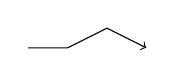
\begin{tikzpicture}[scale=0.5, baseline=(X)]
            \draw[->] (0,0)--(1,0)--(2,0.5)--(3,0);
            \coordinate (X) at (0,0);
        \end{tikzpicture}
        合成给出$(\phi \circ (\psi \circ \theta))_X$。按
        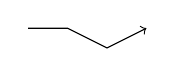
\begin{tikzpicture}[scale=0.5, baseline=(X)]
            \draw[->] (0,0)--(1,0)--(2,-0.5)--(3,0);
            \coordinate (X) at (0,-0.2);
        \end{tikzpicture}
        合成则给出$((\phi \circ \psi) \circ \theta)_X$。这里仍须用上交换图表,结合律证毕。

        最后一个等式可以同样按图索骥。
    \end{proof}
\end{Lem}
    任意函子$F$到自身有恒等态射$\identity_F:F\to F$。给定函子间的态射$\theta:F_1\to F_2$,若态射$\psi:F_2 \to F_1$满足$\psi \circ \theta=\identity_{F_1}, \theta \circ \psi = \identity_{F_2}$,则称$\psi$是$\theta$的逆。可逆的态射称为\emph{函子间的同构},写作$\theta:F_1 \xrightarrow{\sim} F_2$。由定义,若$\theta$的逆存在则唯一,记为$\theta^{-1}$,它无非是在范畴中“逐点地”取逆:$(\theta^{-1})_X:=(\theta_X)^{-1}:F_2X \xrightarrow{\sim}F_1X$。态射$\theta$可逆当且仅当每个$\theta_X$都可逆。易见同构的横纵合成仍是同构。函子间同构$\theta:F_1 \xrightarrow{\sim} F_2$的等价说法是称$\theta_X:F_1 X \xrightarrow{\sim}F_2 X$对变元$X$是\emph{自然同构}或\emph{典范同构}。

\begin{Def}[等价]如果一对函子
    \begin{tikzcd}
        \mathcal{C}_1
            \arrow[bend left = 20, r, "F"] &
        \mathcal{C}_2
            \arrow[bend left = 20, l, "G"]
    \end{tikzcd}
    满足性质:存在函子之间的同构$\theta:FG\xrightarrow{\sim}\identity_{\mathcal{C}_2}, \psi:GF\xrightarrow{\sim}\identity_{\mathcal{C}_1}$
    则称$G$是$F$的\emph{拟逆函子},并称$F$是范畴$\mathcal{C}_1$到$\mathcal{C}_2$的\emph{等价}。
    
    进一步,如果有$FG=\identity_{\mathcal{C}_2},GF=\identity_{\mathcal{C}_1}$,则称$F$是范畴间的\emph{同构},$G$是$F$的\emph{逆}。

    容易证明,等价的合成仍是等价。
\end{Def}
\section{函子范畴}
\section{泛性质}
\section{可表函子}
\section{伴随函子}
\section{极限}
\section{完备性}
\section{习题}